\documentclass[a4paper,12pt]{article}

% Sprachpaket für Deutsch
\usepackage[utf8]{inputenc}
\usepackage[ngerman]{babel}

% Für PDF-Bilder
\usepackage{graphicx}

% Paket für Referenzen
\usepackage{hyperref}
\usepackage[backend=biber, style=numerical]{biblatex}
%Biblatex
\addbibresource{bibtex.bib}
% Titel, Autor und Datum
\title{Brustkrebs Indicatoren}
\author{Timo Michaelis}
\date{\today}

\begin{document}

% Titelbild
\maketitle

\begin{abstract}
Im Folgenden wird versucht anhand verschiedener Indikatoren zur prognostizieren, ob eine Patientin Brustkrebs besitzt.
    Dieses Model dient lediglich der Hilfestellung, nicht aber dem Ersatz eines fachkundigen Arztes
\end{abstract}

\tableofcontents % Inhaltsverzeichnis

\newpage

\section{Einleitung}
In der vorliegenden Arbeit wird eine Unterstützung zur Erkennung von Brustkrebs geboten. Dafür werden verschiedene Eigenschaft
u.a. \textit{durchschnittlicher Radius, durchschnittliche Textur, usw.} berücksichtigt und eine wahrscheinliche Prognose geboten.\newline
Das Ziel dieser Arbeit ist es somit ein Modell zu erstellen, welches bei Input der benötigten Parameter eine vorläufige Diagnose stellt,
welche etwaig dem Patienten bzw. dem Arzt zu einer genaueren Untersuchen verleiten. Dies verringert somit nicht nur die die Chance von
sogenannten \textit{false positives}, sondern kann auch die Bereitschaft unterstützen häufiger notwendige Untersuchungen
durchzuführen, da die Untersuchung weniger komplex wird.\newline
%Literaturarbeit
Im folgenden wird grundsätzlich der Ursprung und Inhalt des Datensatzes diskutiert, sowie die darauf angewandten Methoden näher erläutert.




\section{Datensatz}
Der verwendete Datensatz stammt aus der \textit{Diagnostic Wisconsin Breast Cancer Database.}\textcite{breast_cancer_wisconsin_diagnostic_17}, wie erwartet befasst sich dieser
Datensatz mit Gesundheitlichen Aspekten und besitzt indes folgende \textit{Features}
\begin{itemize}
    \item mean radius
    \item mean texture
    \item mean perimeter
    \item mean area
    \item mean smoothness
    \item mean compactness
    \item mean concavity
    \item mean concave points
    \item mean symmetry
    \item mean fractal dimension
    \item radius error
    \item texture error
    \item perimeter error
    \item area error
    \item smoothness error
    \item compactness error
    \item concavity error
    \item concave points error
    \item symmetry error
    \item fractal dimension error
    \item worst radius
    \item worst texture
    \item worst perimeter
    \item worst area
    \item worst smoothness
    \item worst compactness
    \item worst concavity
    \item worst concave points
    \item worst symmetry
    \item worst fractal dimension
\end{itemize}
Hinzu kommt noch der \textit{Target-Datensatz}, welcher beschreibt ob der Datenpunkt jeweils \textit{Malignand} oder \textit{Benign}
ist.\newline
Bevor näher auf den Datensatz und seine zusammenhänge eingegangen wird, gilt es zu beurteilen inwieweit dieser aufbereitet ist.
Hiefür sei relevant zu testen ob der Datensatz vollständig und inherrent logisch ist, sollte dies nicht der Fall sein, so gilt
es diesen zu bereinigen, durch etwaiges löschen bzw. ersetzen.\newline
Insofern wurde u.a. überprüft ob es null oder negative Werte gibt, solche dürfte es nämlich nicht geben.
Der Datensatz ist frei von solchen Werten, als letzes .\newline
Abseits der Integrität dieses Datensatzes sei noch dessen Koheränz zu überprüfen.
Dafür wurden mehrere Boxplot-Graphen\ref{fig:boxplot1}\ref{fig:boxplot2} erstellt, welche wie ersichtlich Ausreißer angeben, 74 sind insgesamt mit
3$\sigma$ Regel zu finden. Nun gilt es die Frage zu stellen, ob diese Ausreißer entfernt werden müssen.\newline
Letzlich zielt diese Frage darauf ab, ob dieser Algorithmus anwendbar sein kann bzw. soll auf Frauen mit Proportionen außerhalb der Norm und
ob das auschließen das Modell beeinträchtigt. Die Erste Frage lässt sich nur von einem Forscher in dieser Disziplin beantworten,
die Zweite Frage hingegen wird im Fazit wieder betrachtet. Insofern werden die Ausreißer ersteinmal nicht entfernt.
\newline

%code?
Zur Frage ob es Abhängigkeiten zwischen den Features und dem Target gibt, lässt sich dazu eine Grundidee fassen, indem man verschiedene
Features im zwei Dimensionalen gegeneinander aufträgt.\ref{fig:graph}\newline


Ebenfalls lässt sich mittels von Korrellationstabellen ebenfalls Korrellationen\ref{fig:korrelation} nachweisen, weswegen nun nur noch die geignete Methode
zu Erstellung eines Prediction-Algorithmus benötigt wird.
\newline

\section{Methoden}
Es existieren zwei Kategorien in welche unsere Features einsortiert werden, insofern seien Algorithmen notwendig welche eine Klassifikation durchführen.
Für kleinere Datensätze, wie hier vorliegend, ist \textit{ RandomForestClassifier} gut zu nutzen und da bereits aus Graph
eine perfekte lineare separierung nicht möglich ist, ist \textit{SVM (Support Vector Machine)} ebenfalls ein passender Algorithmus zur Modell erstellung.
\subsection{Random Forest Classifier}
Der Random Forest Classifier nutzt eine gewisse Anzahl an verschiedenen Entscheidungsbäumen mit dem Ziel die korrekte Entscheidung zu erfüllen,
dies führt dazu, dass die Nachteile eines Entscheidungsbaumes verringert (wie z.B. \textit{overfitting})
\subsection{Support Vector Machine}
Ein SVM nutzt die Tatsache aus, dass selbst wenn eine Separierbarkeit z.B. im 2-Dimensionalen nicht machbar ist,
diese in höheren Dimensionen durchaus möglich ist.
\subsubsection{Kernel}
\begin{itemize}
    \item \textbf{rbf} Die gängigste Methode
    \item \textbf{linear} Dies diente mehr zur Überprüfung, ob dieses Problem nicht auch durch eine lineare Separierung teilbar ist.\newline
    Wie aber hier zusehen, ist diese Lösung nicht optimal
    \item \textbf{poly}
\end{itemize}
\section{Ergebnisse}
Um das bestmöglichste Ergebnis zu erzielen, wurde ein Grid angewandt damit die bessere Anzahl an Entscheidungsbäumen bzw.
des Wertes der Fehlklassifizierungsstrafe genutzt werden kann. Im folgenden werden die Modelle mitsamt ihrer Güte vorgestellt.
\subsection{Random Forest Classifier}
Für die Wahl der Anzahl an Bäumen ist laut der Gridanalyse\ref{fig:gcforest}, 200 am passendsten, weitere Optimierungen seien zwar möglich, nicht aber zielführend,
da höhere Genauigkeiten signifikant mehr Rechenzeit benötigen würden.\newline

Zur Erstellung des Modells mittels des \textit{Random Forest Classifiers} wurden die Daten in zwei Teile unterschieden, da 30\% der Daten als
Testdaten dienen sollen. Da leider nicht übermäßig viele Daten vorliegen, der Datensatz ist kleiner als tausend, sollte der Testdaten Anteil zumindest
über 150 liegen.\newline
Mit diesen Eigenschaften ergab sich eine Accuracy von 0.9708 und eine Precision von 0.9725. Im Vergleich dazu besaß das Modell
mit nur 10 Entscheidungsbäumen eine Accuracy von 0.9532 und eine Precision von 0.9630.\newline
Veranschaulicht wird die Güte dieses Modells auch noch mittels einer Confusion Matrix\ref{fig:confforest}, welche die Fehlklassifikation von false positives bzw. false
negatives zeigt.\newline


\subsection{Support Vector Machine}
Für die passende Wahl an Parameter der Support Vector Machine gibt es zwei Parameter welche die größte Signifikanz besitzen, zum einen
die Fehlklassifizierungsstrafe aber auch die passende Kernelmethode, ersichtlich in der Graphik\ref{fig:gcsvm} ist die passende Fehlklassifizierungsstrafe
100. Für die passende Wahl der Kernelmethode ist ausprobieren meist die schnellste Methode

\begin{itemize}
    \item \textbf{rbf} Die gängigste Methode sie ergab 0.9708 Accuracy sowie 0.9722 Precision und ebenfalls eine ähnlich confusion Matrix\ref{fig:confsvmrbf}

    \item \textbf{linear} Diese Methode ergab 0.9766 Accuracy sowie 0.9905 Precision und ebenfalls eine ähnlich confusion Matrix\ref{fig:confsvmlinear}.\newline

    \item \textbf{poly} Diese Methode ergab 0.9649 Accuracy sowie 0.9550 Precision und ebenfalls eine ähnlich confusion Matrix\ref{confsvmpoly.png}.\newline

\end{itemize}
\section{Diskussion}
Beide Systeme besitzen zwar ähnliche Akkuratheit, dennoch besitzt das SVM Modell mit linearem Kernel die höchste Akkuratheit, sowie die höchste
Precision. Stellt man die beiden Gegenüber\ref{fig:vergleich} wird eine kleine Überlegenheit des SVM Modells sichtbar.

\section{Fazit}
Generell erlaubt dieses Modell nun eine recht akkurate Einschätzung von Brustkrebs, mangels allzu umfangreicher Datenmenge sei dies
aber nur mit Vorsicht zu genießen. Zusätzlich besitzt trotz der Außreiser
\newpage

% Anhang für das Jupyter Notebook
\appendix
\section{Anhang: Erklärung}
\section{Anhang: Grafiken}
\begin{figure}[H]
    \centering
    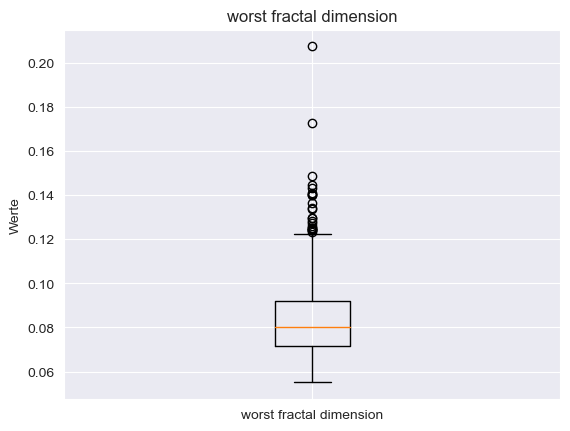
\includegraphics[width=\textwidth]{boxplot1.png}
    \caption{Boxplot der worst fractal Dimension}
    \label{fig:boxplot1}
\end{figure}
\begin{figure}[H]
    \centering
    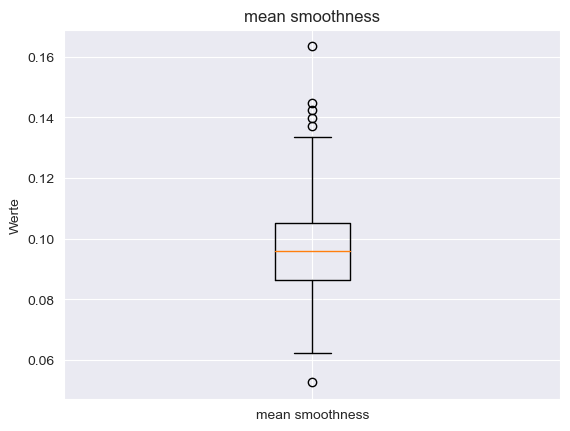
\includegraphics[width=\textwidth]{boxplot2.png}
    \caption{Boxplot der mean smoothness}
    \label{fig:boxplot2}
\end{figure}
\begin{figure}[H]
    \centering
    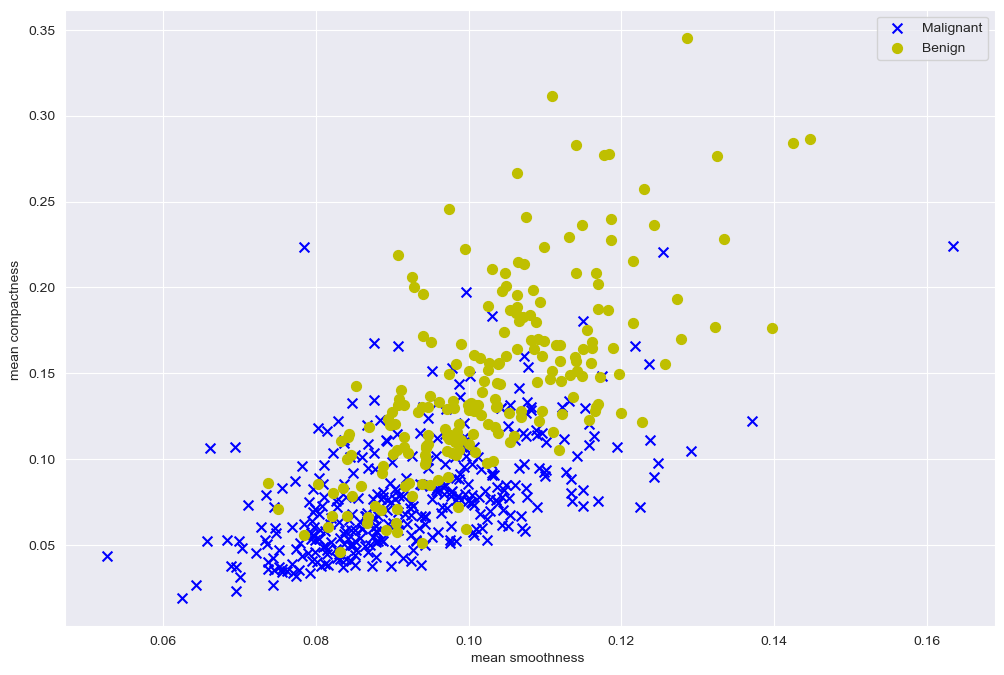
\includegraphics[width=\textwidth]{graph.png}
    \caption{Mean smoothness und mean compactness}
    \label{fig:graph}
\end{figure}
\begin{figure}[H]
    \centering
    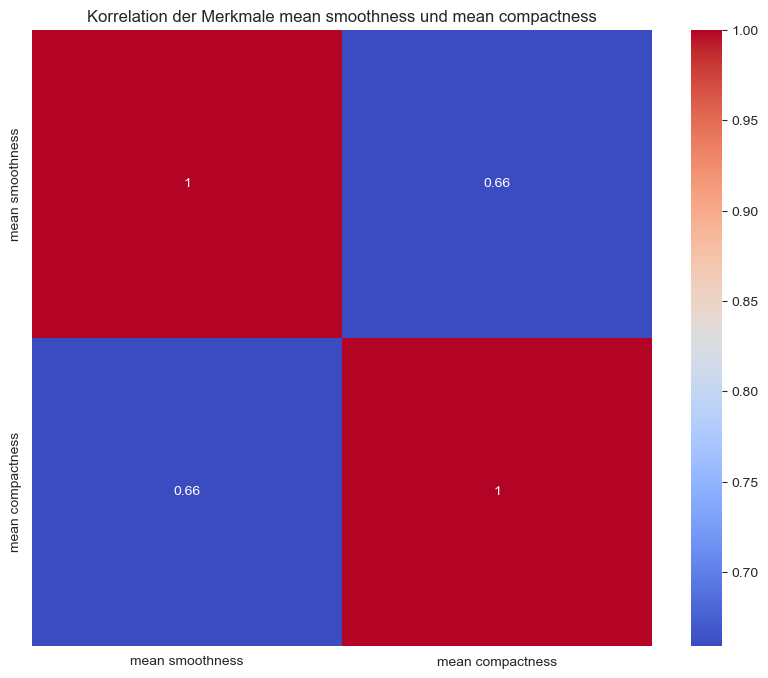
\includegraphics[width=\textwidth]{korrelation.png}
    \caption{Korelation von }
    \label{fig:korrelation}
\end{figure}
\begin{figure}[H]
    \centering
    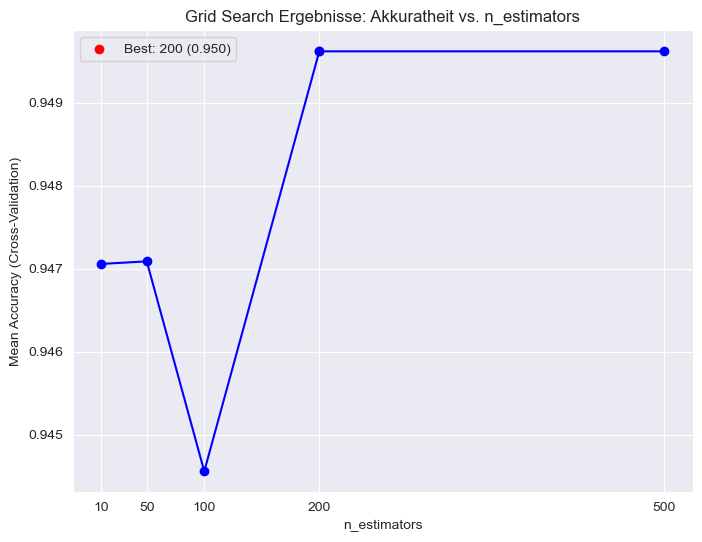
\includegraphics[width=\textwidth]{gridcodeForest.png}
    \caption{Jupyter Notebook als Anhang}
    \label{fig:gcforest}
\end{figure}
\begin{figure}[H]
    \centering
    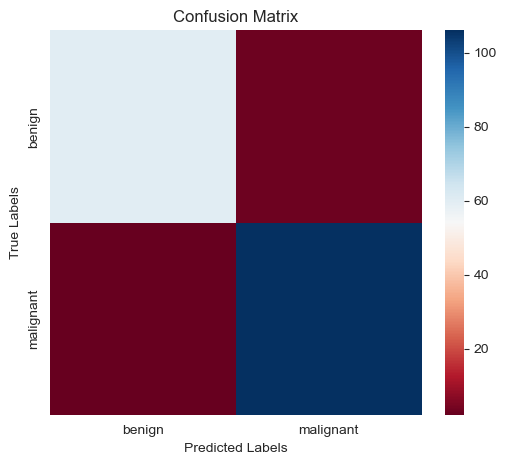
\includegraphics[width=\textwidth]{confforest.png}
    \caption{Jupyter Notebook als Anhang}
    \label{fig:confforest}
\end{figure}
\begin{figure}[H]
    \centering
    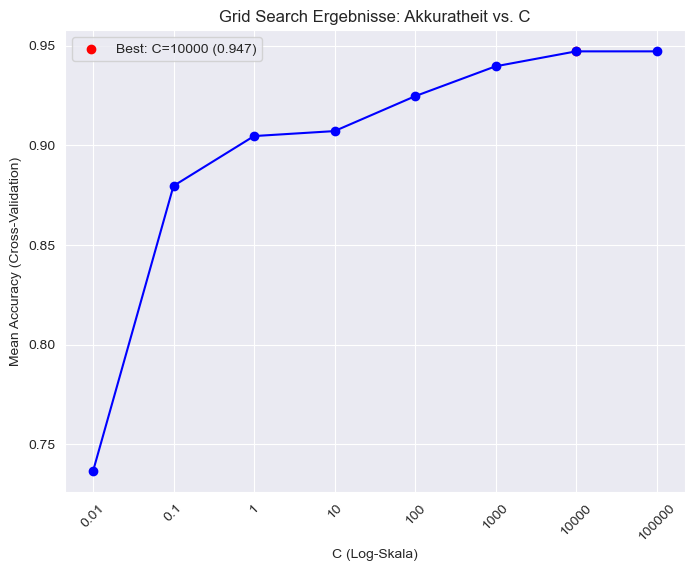
\includegraphics[width=\textwidth]{gridcodesvm.png}
    \caption{Jupyter Notebook als Anhang}
    \label{fig:gcsvm}
\end{figure}
\begin{figure}[H]
    \centering
    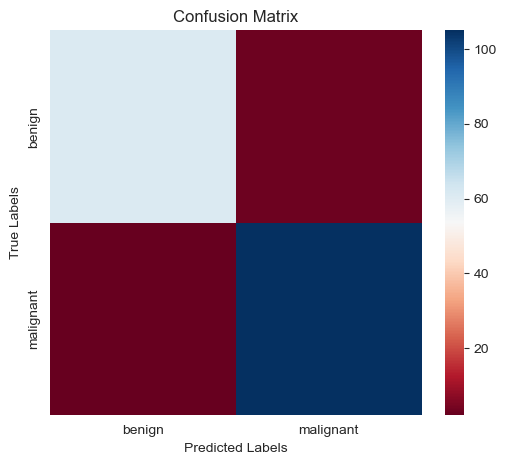
\includegraphics[width=\textwidth]{confsvmrbf.png}
    \caption{Jupyter Notebook als Anhang}
    \label{fig:confsvmrbf}
\end{figure}
\begin{figure}[H]
    \centering
    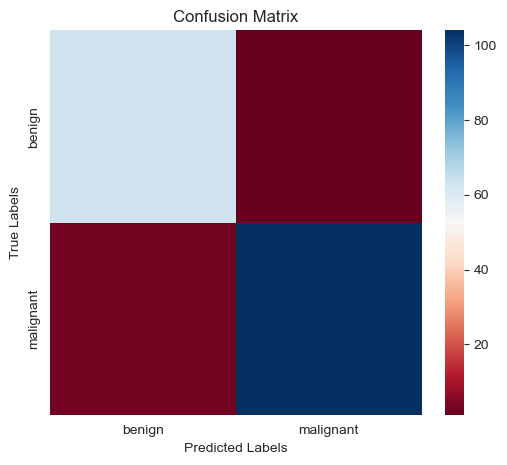
\includegraphics[width=\textwidth]{confsvmlinear.png}
    \caption{Jupyter Notebook als Anhang}
    \label{fig:confsvmlinear}
\end{figure}
\begin{figure}[H]
    \centering
    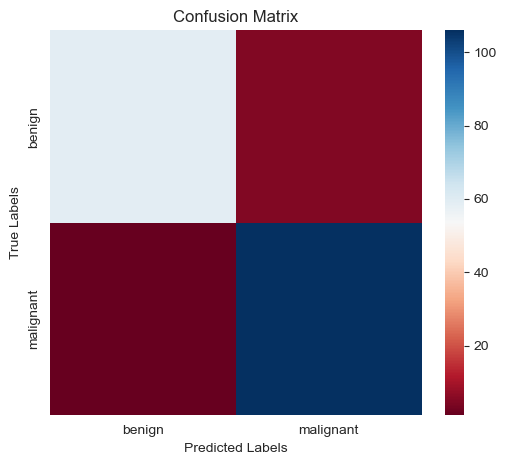
\includegraphics[width=\textwidth]{confsvmpoly.png}
    \caption{Jupyter Notebook als Anhang}
    \label{fig:confsvmpoly}
\end{figure}
\begin{figure}[H]
    \centering
    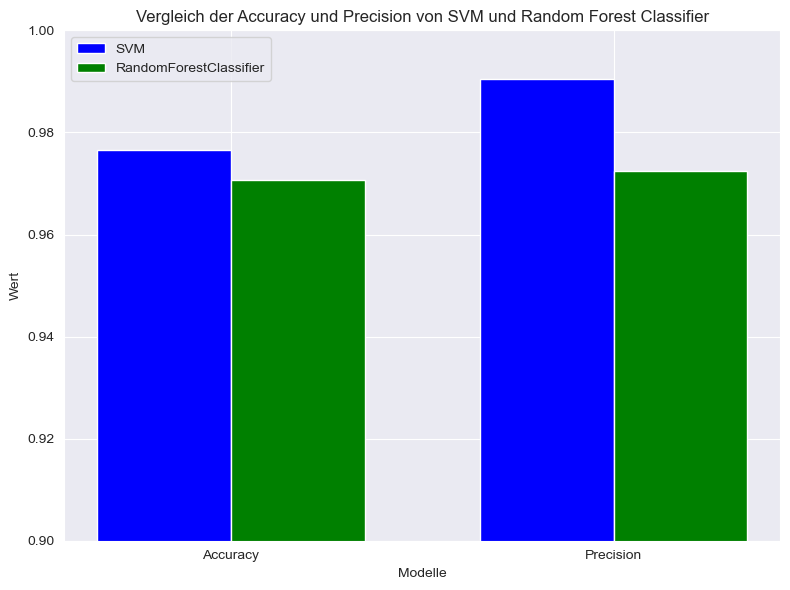
\includegraphics[width=\textwidth]{vergleich.png}
    \caption{Vergleich der Accuracy und Precision von SVM und Random Forest Classifier}
    \label{fig:vergleich}
\end{figure}
\end{document}
